
\section*{Energy Calibration}

Due to the organic composition of our detectors the photoelectric cross section of its constituents is negligible in the energy range considered. Furthermore total absorption through multiple Compton scattering is negligible too, because of detector limited size . The detectors response will be dominated by individual Compton interaction, thus the energy spectrum is a continuous distribution that corresponds to different angles of interaction. This can be seen in the spectra acquired with the $^{22}$Na source in Fig. \ref{fig: uncalibrated energy spectra}.

\begin{figure}[h!]
\centering
\subfloat[][\emph{Detector 1 }.]
   {\includegraphics[width=.45\textwidth]{d1_spectrum_qlong}} \quad
\subfloat[][\emph{Detector 2 }.]
   {\includegraphics[width=.45\textwidth]{d2_spectrum_qlong}} \\
\caption{\emph{Detector 1} (a) and \emph{Detector 2} (b) uncalibrated energy spectra  obtained from a $^{22}$Na $\gamma$-source.}
\label{fig: uncalibrated energy spectra}
\end{figure}

The finite resolution of our detectors results in a shift towards lower energies depending on the detector resolution as shown in Fig.~\ref{fig: smeared spectra}.
\begin{figure}[h!]
\centering
\includegraphics[width=0.8\textwidth]{smeared_spectra}
\caption{Gaussian smeared spectra at different $\sigma$ generated using the  Klein-Nishina Compton scattering cross section  for 511~keV photons.}
\label{fig: smeared spectra}
\end{figure}

In order to obtain the energy calibration parameters, several smeared spectra were generated using the  Klein-Nishina Compton scattering cross section~(see Eq.~\ref{eq:Klein-Nishina}) for $511$ keV and $1275$ keV $\gamma$ respectively.
\begin{equation}
\dfrac{d\sigma}{dT} = \dfrac{\pi r_e^2}{m_ec^2\alpha^2}\left(2+\dfrac{s^2}{\alpha^2(1-s)^2}+\dfrac{s}{1-s} \left(s-\dfrac{2}{\alpha}\right) \right)
\label{eq:Klein-Nishina}
\end{equation}
%To locate the Compton edge then, the background from acquired spectra was removed  as shown in Fig.~\ref{fig: compton back}.
%\begin{figure}[h!]
%\centering
%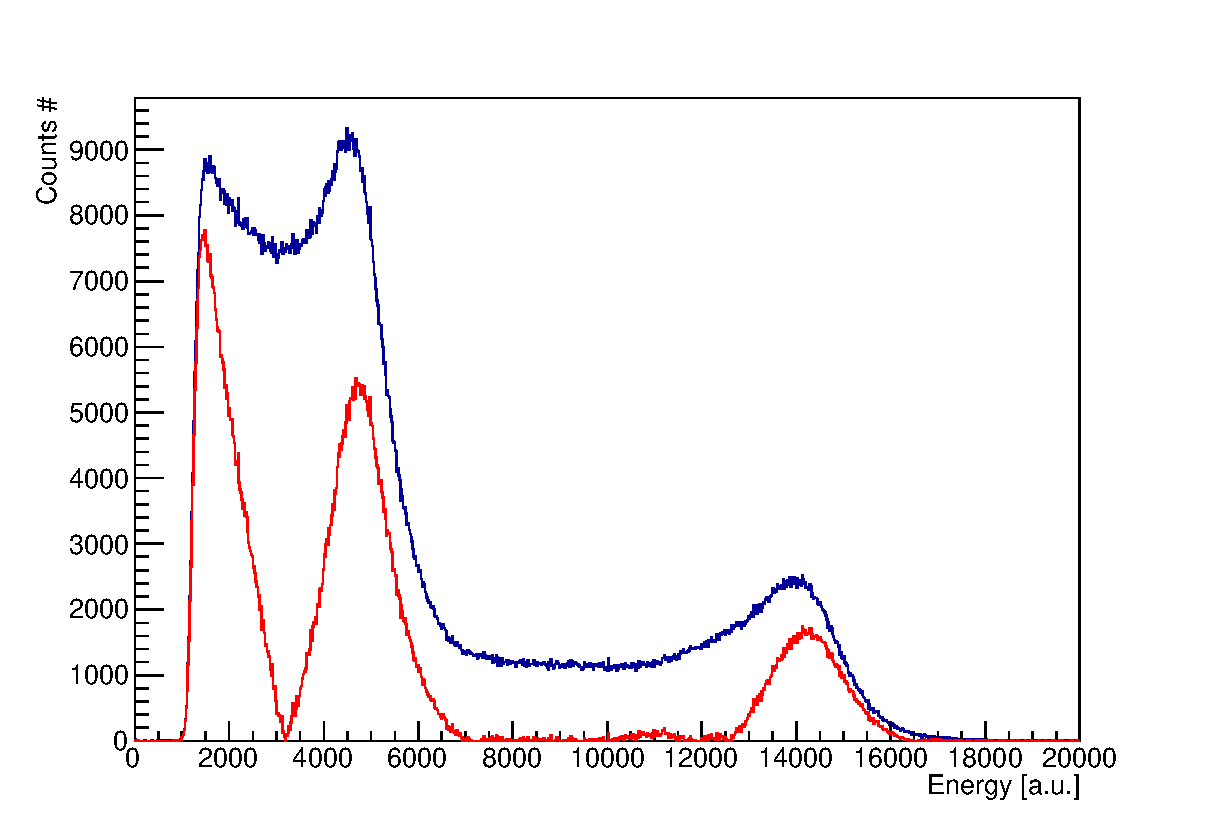
\includegraphics[width=0.8\textwidth]{spectra_vs_background.eps}
%\caption{$^{22}$Na energy spectra. The blue one represent the original acquired spectrum, while the red one is obtained by background removal.}
%\label{fig: compton back}
%\end{figure}
The $\chi^2$ between experimental spectrum and Gaussian smeared spectra was minimized looping over different $\sigma$ values. With the selected $\sigma$ the corresponding shift of the Compton edge was computed in order to calibrate the detectors as shown in Tab.~\ref{tab:CEshift}:

\begin{table}[h!]
	\centering
	\begin{tabular}{ccccc}
		\toprule
		\toprule
		Detector & Photon Energy [keV] & $\sigma$ [keV] & Resolution & C.E. shifting [keV] \\
		\midrule
		1&511    & 34 & $11\%$ & 40.66 \\
		  &1275 & 40 & $4\%$  & 52.15   \\
		\midrule
		2&511   & 28  & $9\%$& 34.66 \\
		  &1275 & 40 & $4\%$& 52.15  \\
		\bottomrule
		\bottomrule
	\end{tabular}
	\caption{$\sigma$, Resolution and C.E. shift for the two detectors.}
	\label{tab:CEshift}
\end{table}
\newpage
Finally the calibration parameters were computed~(see Tab.~\ref{tab:Cal_par}), the $^{22}$Na  calibrated spectra of the two detectors are shown in Fig.~\ref{fig: calibrated energy spectra}

\begin{table}[h!]
	\centering
	\begin{tabular}{ccc}
		\toprule
		\toprule
		Detector & a [keV/channel] & b [keV] \\
		\midrule
		\#1 &  0.07 & -54.3 \\
		\#2 & 0.08 & -32.7 \\
		\bottomrule
		\bottomrule
	\end{tabular}
	\caption{Calibration parameters.}
	\label{tab:Cal_par}
\end{table}

\begin{figure}[h!]
\centering
\subfloat[][\emph{Detector 1}.]
   {\includegraphics[width=.45\textwidth]{calibrated_spectra_d1}} \quad
\subfloat[][\emph{Detector 2}.]
   {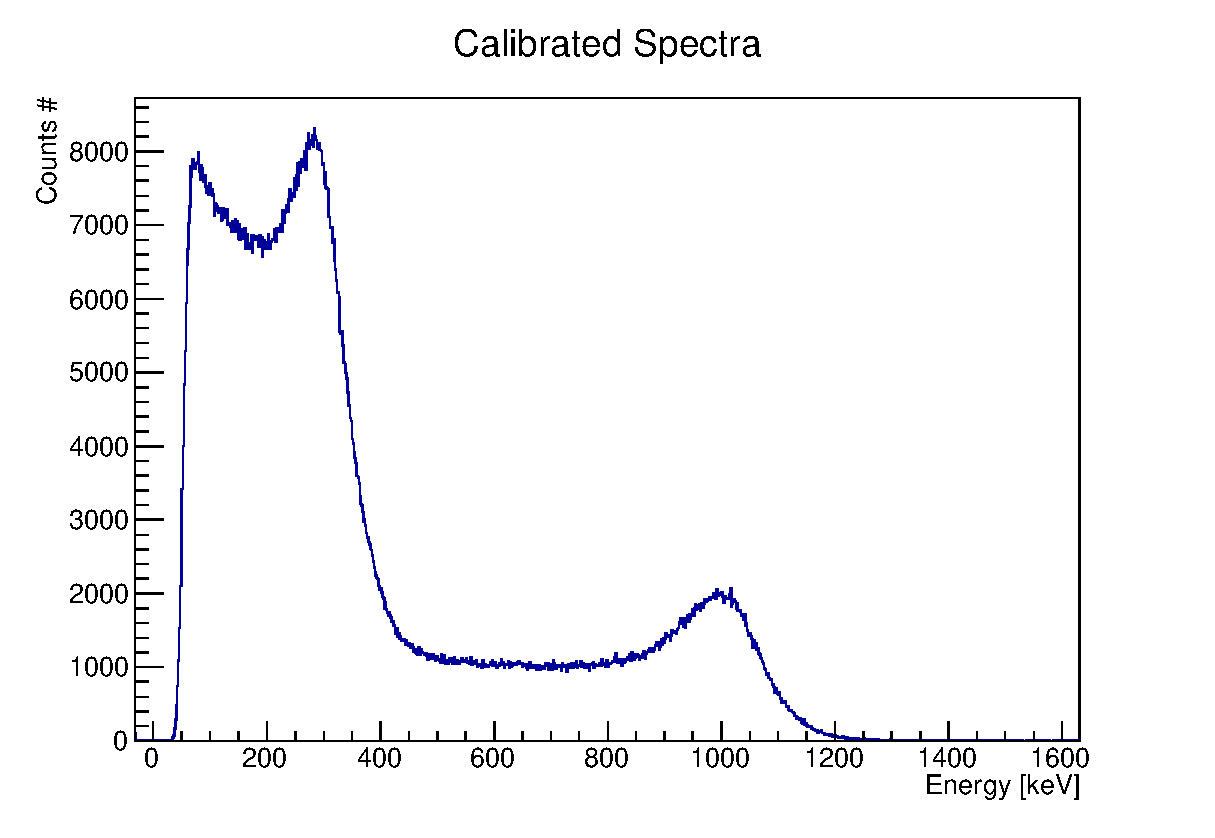
\includegraphics[width=.45\textwidth]{calibrated_spectra_d2}} \\
\caption{\emph{Detector 1} (a) and \emph{Detector 2} (b) energy calibrated spectra  obtained from a $^{22}$Na $\gamma$ source.}
\label{fig: calibrated energy spectra}
\end{figure}

\clearpage
\section*{TAC Calibration}
In order to calibrate the TAC unit, several spectra were produced using as start input the CFD timing signals and as stop the same signals delayed by a chosen value. With 2~ns delay steps the spectra of Fig. \ref{fig: uncalibrated TAC} was obtained, the peaks centroids were used to compute the calibration parameters performing a linear fit~(see Fig.~\ref{fig: fit tac}). 
\begin{figure}[h!]
\centering
\includegraphics[width=0.8\textwidth]{tac_uncalibrated_spectrum.pdf}
\caption{TAC uncalibrated spectrum obtained by an auto coincidence with 2~ns delay steps. }
\label{fig: uncalibrated TAC}
\end{figure}


\begin{figure}[h!]
\begin{minipage}[b]{0.6\textwidth}
\centering
\includegraphics[width=\textwidth]{fit_calibrazione_tac}
\caption{Linear fit used to compute the TAC calibration parameters.}
\label{fig: fit tac}
\end{minipage}
\hfill
\begin{minipage}[b]{0.45\textwidth}
\centering
\begin{tabular}{cc}
\toprule
\toprule
Parameter & Value \\
\midrule
p0     & (-1.19 $\pm$  0.04) s \\
p1     & (7.36   $\pm$  0.01)$\times 10^{-4}$ s/ch\\
\bottomrule
\bottomrule
\end{tabular}
\vspace{1.5cm}
\caption*{Fit parameters.}
\end{minipage}
\end{figure}
\newpage

